\documentclass[11pt, oneside]{article}   	% use "amsart" instead of "article" for AMSLaTeX format
\usepackage{geometry}                		% See geometry.pdf to learn the layout options. There are lots.
\geometry{letterpaper}                   		% ... or a4paper or a5paper or ... 
%\geometry{landscape}                		% Activate for rotated page geometry
%\usepackage[parfill]{parskip}    		% Activate to begin paragraphs with an empty line rather than an indent
\usepackage{graphicx}				% Use pdf, png, jpg, or eps§ with pdflatex; use eps in DVI mode
								% TeX will automatically convert eps --> pdf in pdflatex		
\usepackage{amssymb}
\usepackage[T1]{fontenc}
\usepackage{mwe}    % loads �blindtext� and �graphicx�

\usepackage{caption}
\usepackage{float}
\usepackage{subcaption}

%SetFonts

%SetFonts


\title{% 
	CS5487 Programming Assignment 1 \\ 
			Report}
\author{LIN Jiecong (54938833)}
%\date{}							% Activate to display a given date or no date

\begin{document}
\maketitle


\section{Polynomial function}
\subsection{Well-working Hyperparameter Selection}
\begin{figure}[H]
\centering
\begin{subfigure}{.3\textwidth}
  	\centering
  	\includegraphics[width=.9\linewidth]{bayesian_param.eps}
  	\caption{Bayesian Regression}
  	\label{fig:sub1}
\end{subfigure}%
\begin{subfigure}{.3\textwidth}
  	\centering
  	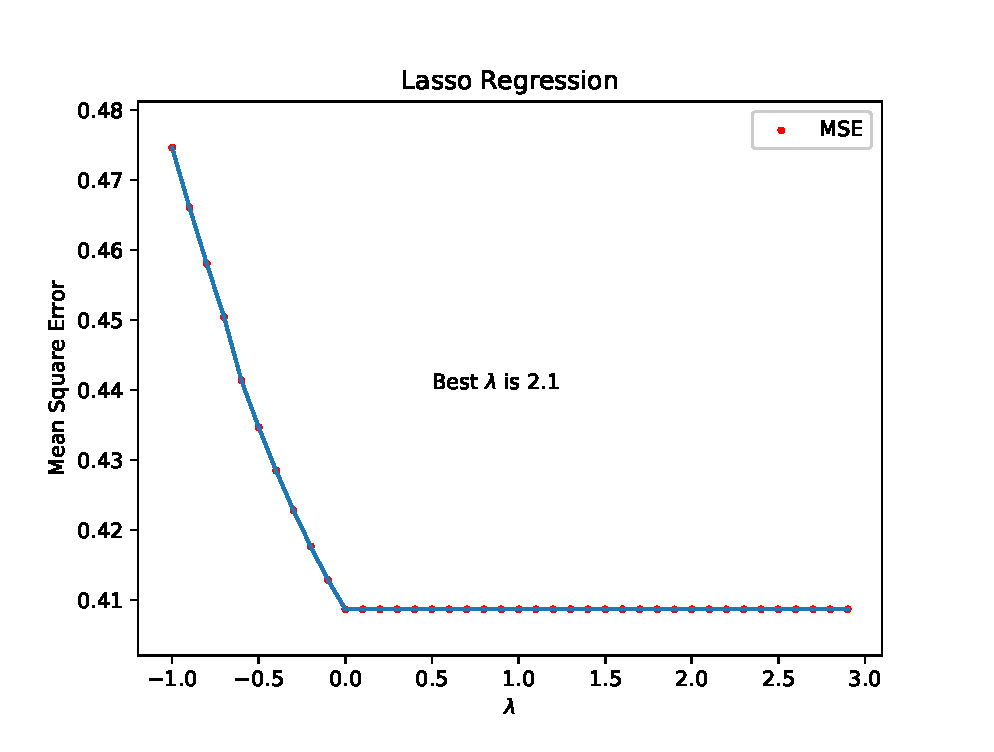
\includegraphics[width=.9\linewidth]{lasso_param.eps}
  	\caption{Lasso Regression}
  	\label{fig:sub2}
\end{subfigure}%
\begin{subfigure}{.3\textwidth}
  	\centering
  	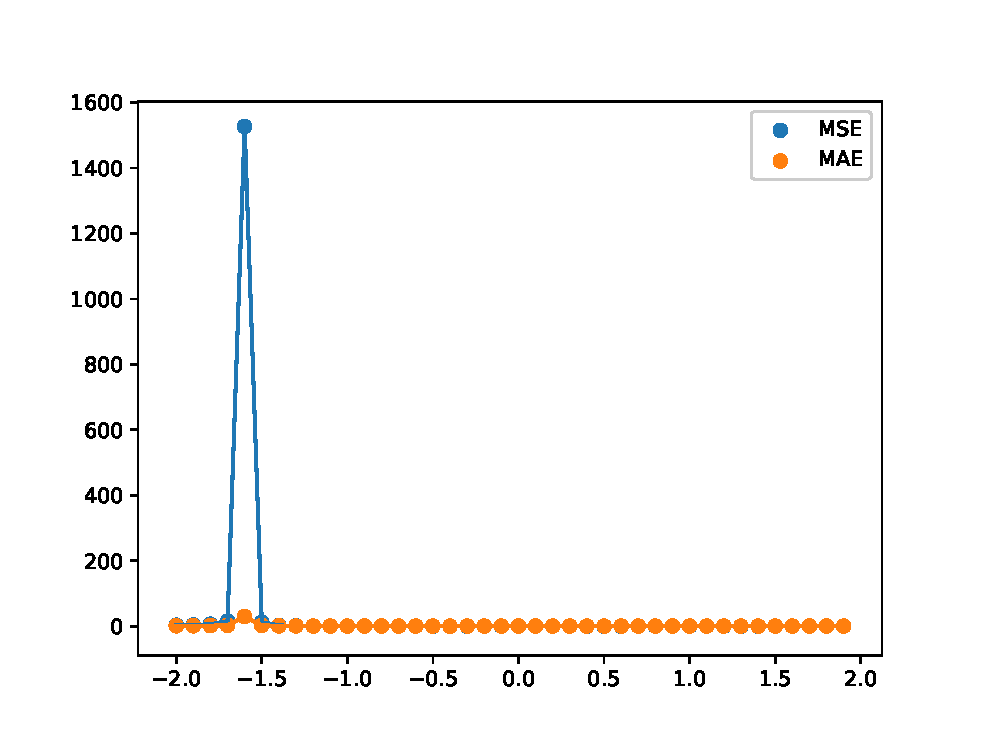
\includegraphics[width=.9\linewidth]{ls_param.eps}
  	\caption{Regularized LS Regression}
  	\label{fig:sub2}
\end{subfigure}
	\caption{Mean Squres Error Based on Different Hyperparameters }
	\label{fig:param}
\end{figure}

For each regression method, experiments used the sample data (\emph{samplx, sampley})  to estimate the parameters of a 5th order polynomial function. Firstly, I have done several experiments to select best hyperparameters for BR, RLS and LASSO. 

For both RLS and LASSO, I used $\lambda \in [-1.0, 3.0]$ for regression based on sample data (\emph{samplx, sampley}), then using \emph{polyx} to predict the output and calculating the mean-squared error. As for Bayesian Regression, testing $\alpha$ was generated from $[0.1, 20.0]$. The experiment results (see figure \ref{fig:param})show that the best hyperparameters of three regression model are $\lambda = 0.5$(Regularized LS Regression), $\lambda=2.1$(Lasso Regression) and $\alpha=10.4$(Bayesian Regression). In the following experiment, these three best hyperparameters will be used for regression.

\subsection{Regression and Prediction on Original Samples}

In this part, I implemented 5 regression algorithm for the 5th order polynomial. For each regression method, use the sample data (\emph{sampx, sampy}) to estimate the parameters of a 5th order polynomial function. Figure \ref{fig:5th} shows the estimated function using polyx as inputs, along with the sample data. For BR, I also plot the standard deviation around the mean (see Figure \ref{fig:br5}).

\begin{table}[htp]
\caption{Mean Square Error}
\begin{center}
\begin{tabular}{|c|c|}
\hline
		Algorithm  &  MSE \\
\hline	
		Least Square    &  0.4086 \\
		Regularized LS &  0.4076 \\
		Lasso		&  0.4086 \\
		Robust		&  0.7680 \\
		\textbf{Bayesian}& 0.4075 \\
\hline
\end{tabular}
\end{center}
\label{default}
\end{table}%

From the experiment we can see that the regression lines generated by 5 algorithms can well fit the sample data, among them Bayesian Regression gains the least MSE Score (MSE=0.4075) and Robust Regression gains the larger one (MSE=0.768). LS, RLS and BR achieved almost the same performance while Robust Regression has the worst performance on sample data apparently. 

\begin{figure}[H]
\centering
\begin{subfigure}{.3\textwidth}
  	\centering
  	\includegraphics[width=.9\linewidth]{BayessianRegression_5thorder.eps}
  	\caption{Bayesian Regression}
  	\label{fig:br5}
\end{subfigure}%
\begin{subfigure}{.3\textwidth}
  	\centering
  	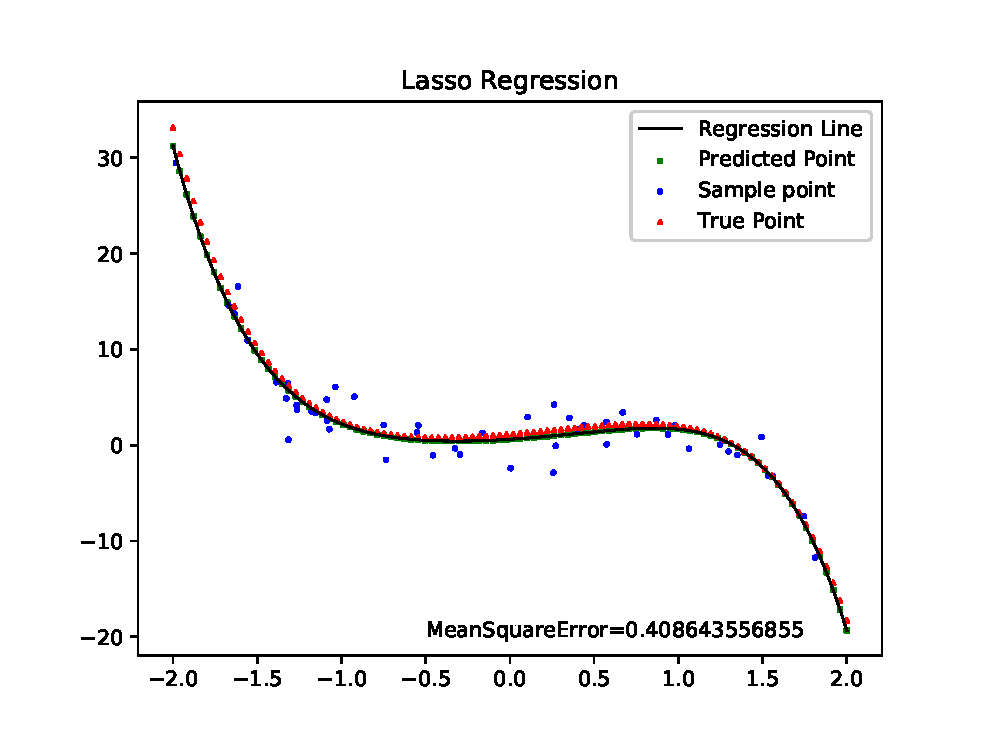
\includegraphics[width=.9\linewidth]{LassoRegression_5thorder.eps}
  	\caption{Lasso Regression}
  	\label{fig:sub2}
\end{subfigure}
\begin{subfigure}{.3\textwidth}
  	\centering
  	\includegraphics[width=.9\linewidth]{LeastSquareRegression_5thorder.eps}
  	\caption{Least Square Regression}
  	\label{fig:}
\end{subfigure}%
\begin{subfigure}{.3\textwidth}
  	\centering
  	\includegraphics[width=.9\linewidth]{RobustRegression_5thorder.eps}
  	\caption{Robust Regression}
  	\label{fig:sub2}
\end{subfigure}%
\begin{subfigure}{.3\textwidth}
  	\centering
  	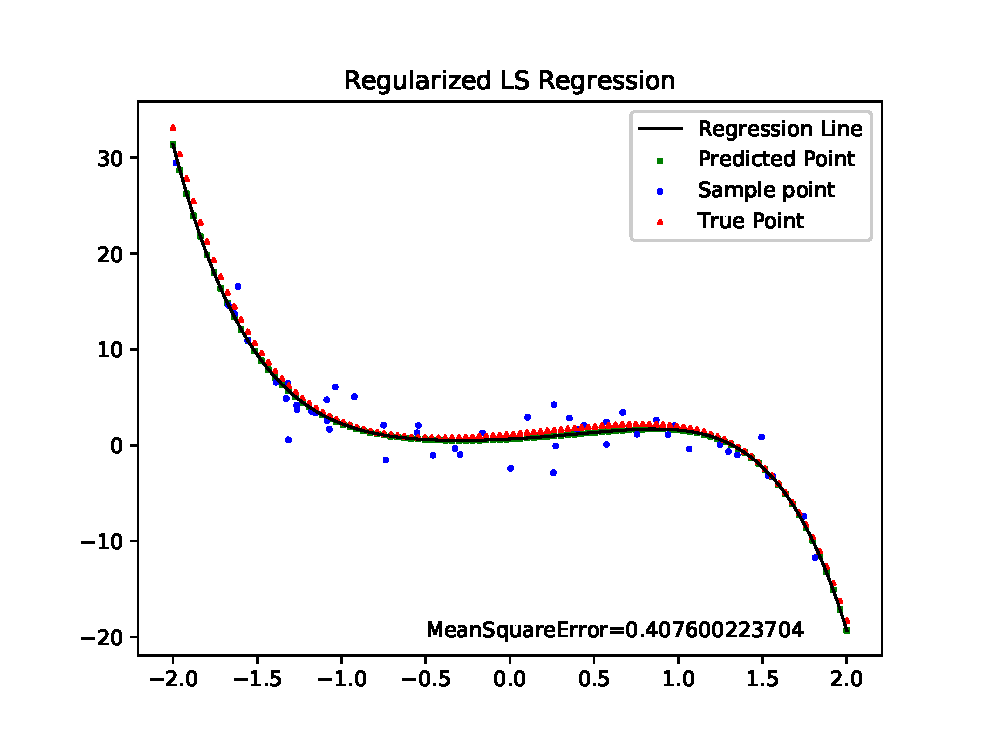
\includegraphics[width=.9\linewidth]{RegularizedLSRegression_5thorder.eps}
  	\caption{Regularized LS Regression}
  	\label{fig:rls}
\end{subfigure}
	\caption{Regression and Prediction of 5 algorithms}
	\label{fig:5th}
\end{figure}

\subsection{Regression and Prediction on Subset of Samples}

In this part, my experiment reduces the amount of training data available by selecting some subsets of the sample. I generated 9 kinds of subsets whose size ranges from 15\% to 95\%, then I  ran experiment 2000 times on every single subset and calculated the average MSE.

\begin{figure}[H]
\centering
\begin{subfigure}{.18\textwidth}
  	\centering
  	\includegraphics[width=.9\linewidth]{BayesianRegression_outliers15.eps}
  	\caption{15\%}
\end{subfigure}%
\begin{subfigure}{.18\textwidth}
  	\centering
  	\includegraphics[width=.9\linewidth]{BayesianRegression_outliers25.eps}
  	\caption{25\%}
\end{subfigure}%
\begin{subfigure}{.18\textwidth}
  	\centering
  	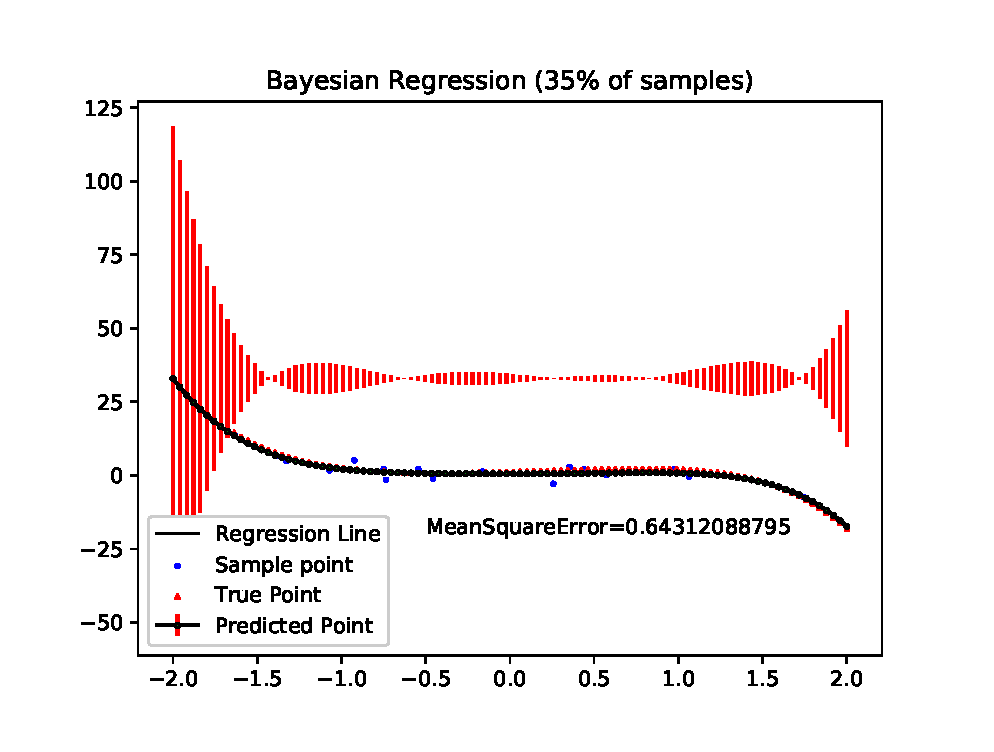
\includegraphics[width=.9\linewidth]{BayesianRegression_outliers35.eps}
  	\caption{35\%}
\end{subfigure}%
\begin{subfigure}{.18\textwidth}
  	\centering
  	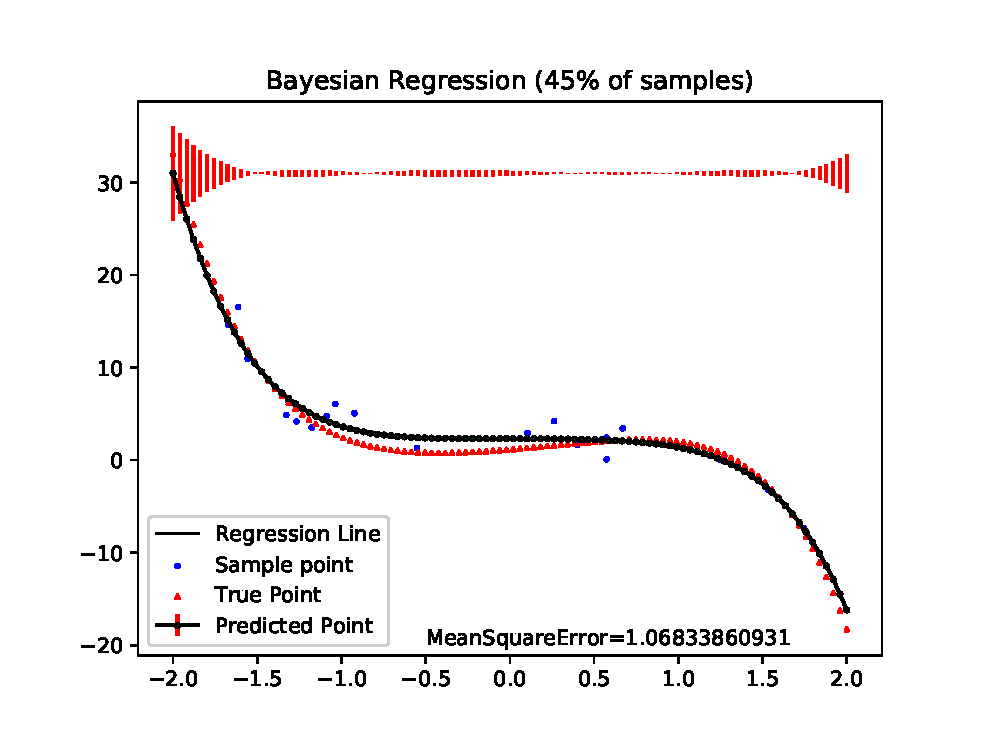
\includegraphics[width=.9\linewidth]{BayesianRegression_outliers45.eps}
  	\caption{45\%}
\end{subfigure}
\begin{subfigure}{.18\textwidth}
  	\centering
  	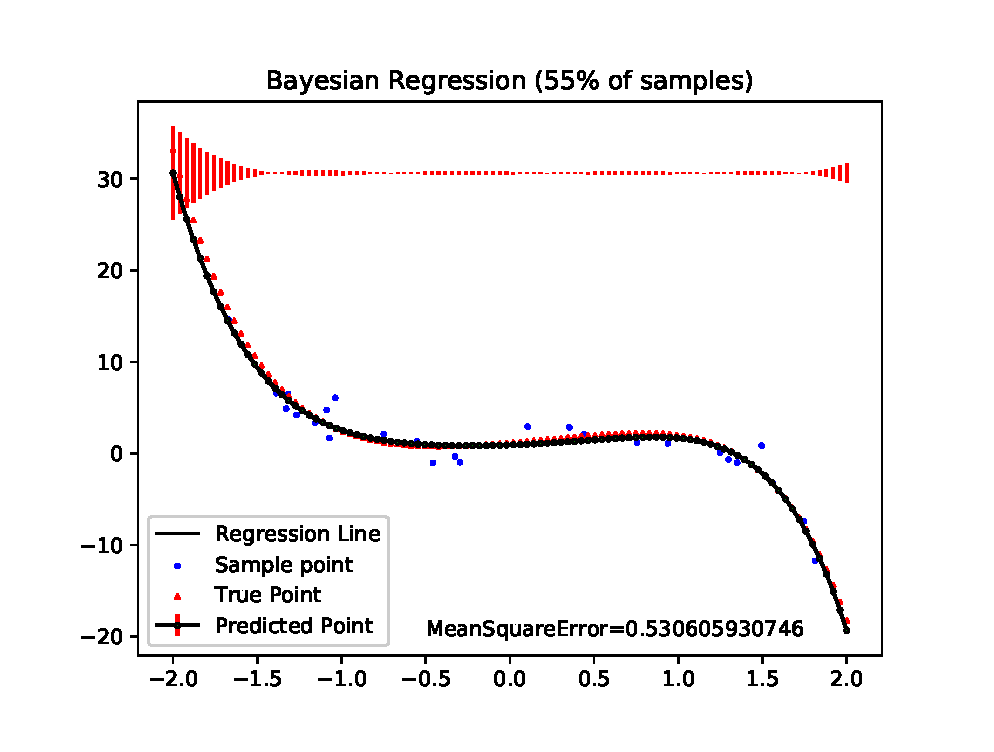
\includegraphics[width=.9\linewidth]{BayesianRegression_outliers55.eps}
  	\caption{45\%}
\end{subfigure}%
\begin{subfigure}{.18\textwidth}
  	\centering
  	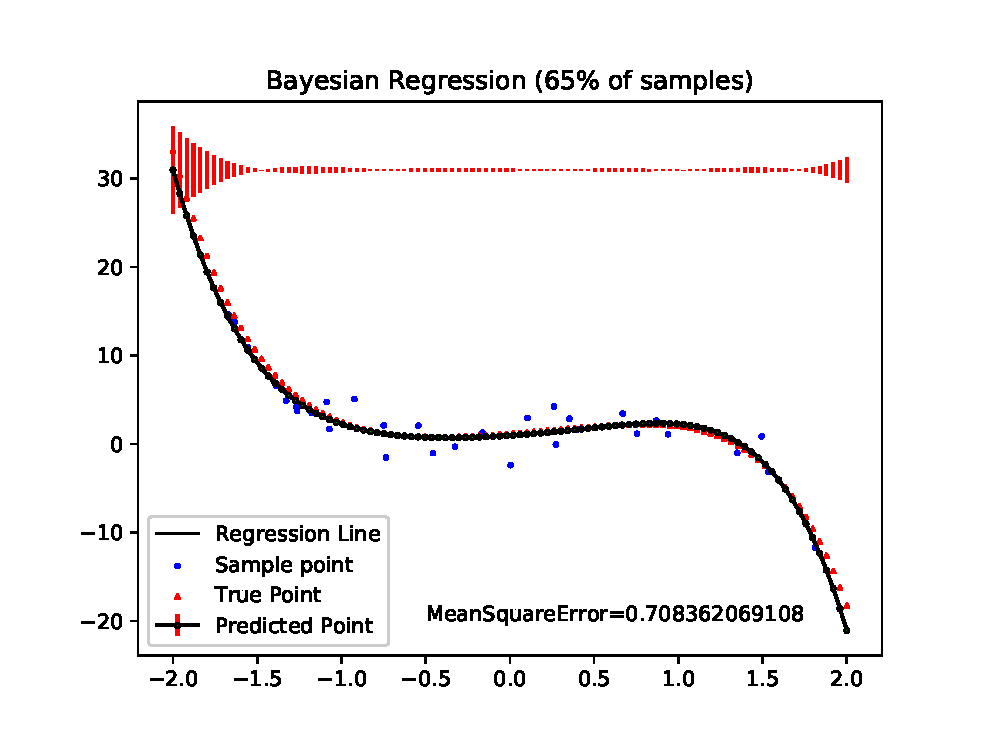
\includegraphics[width=.9\linewidth]{BayesianRegression_outliers65.eps}
  	\caption{65\%}
\end{subfigure}%
\begin{subfigure}{.18\textwidth}
  	\centering
  	\includegraphics[width=.9\linewidth]{BayesianRegression_outliers75.eps}
  	\caption{75\%}
\end{subfigure}%
\begin{subfigure}{.18\textwidth}
  	\centering
  	\includegraphics[width=.9\linewidth]{BayesianRegression_outliers85.eps}
  	\caption{85\%}
\end{subfigure}%
\begin{subfigure}{.18\textwidth}
  	\centering
  	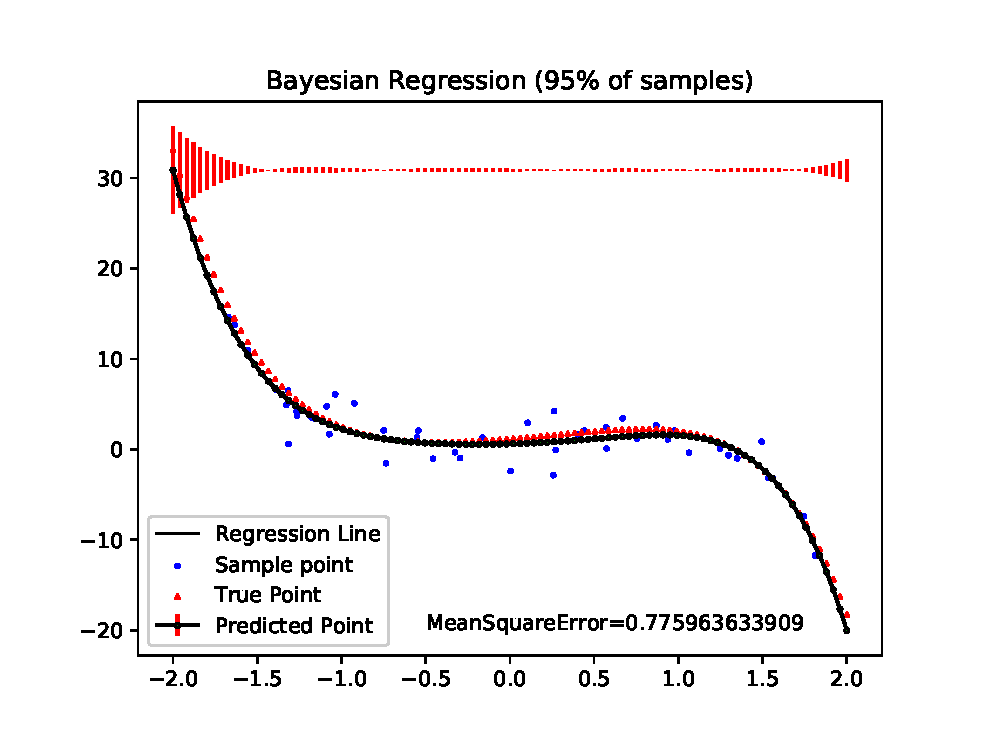
\includegraphics[width=.9\linewidth]{BayesianRegression_outliers95.eps}
  	\caption{95\%}
\end{subfigure}
	\caption{Bayesian Regression}
\end{figure}

\begin{figure}[H]
\centering
\begin{subfigure}{.18\textwidth}
  	\centering
  	\includegraphics[width=.9\linewidth]{LassoRegression_outliers15.eps}
  	\caption{15\%}
\end{subfigure}%
\begin{subfigure}{.18\textwidth}
  	\centering
  	\includegraphics[width=.9\linewidth]{LassoRegression_outliers25.eps}
  	\caption{25\%}
\end{subfigure}%
\begin{subfigure}{.2\textwidth}
  	\centering
  	\includegraphics[width=.9\linewidth]{LassoRegression_outliers35.eps}
  	\caption{35\%}
\end{subfigure}%
\begin{subfigure}{.18\textwidth}
  	\centering
  	\includegraphics[width=.9\linewidth]{LassoRegression_outliers45.eps}
  	\caption{45\%}
\end{subfigure}
\begin{subfigure}{.18\textwidth}
  	\centering
  	\includegraphics[width=.9\linewidth]{LassoRegression_outliers55.eps}
  	\caption{45\%s}
\end{subfigure}%
\begin{subfigure}{.2\textwidth}
  	\centering
  	\includegraphics[width=.9\linewidth]{LassoRegression_outliers65.eps}
  	\caption{65\%}
\end{subfigure}%
\begin{subfigure}{.18\textwidth}
  	\centering
  	\includegraphics[width=.9\linewidth]{LassoRegression_outliers75.eps}
  	\caption{75\%}
\end{subfigure}%
\begin{subfigure}{.18\textwidth}
  	\centering
  	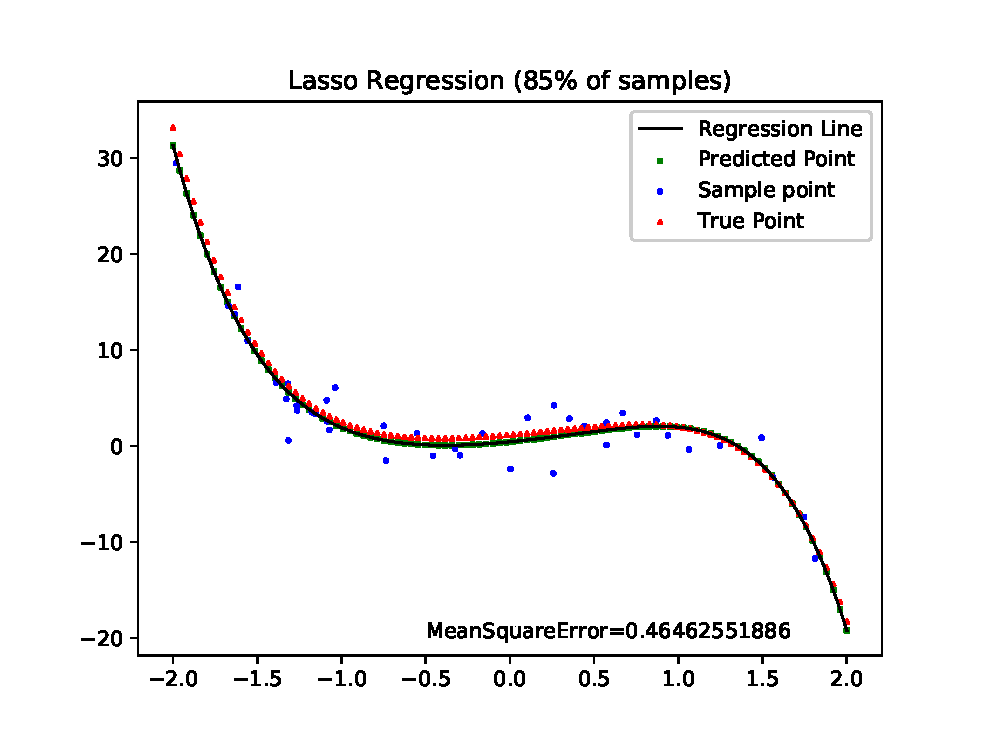
\includegraphics[width=.9\linewidth]{LassoRegression_outliers85.eps}
  	\caption{85\%}
\end{subfigure}%
\begin{subfigure}{.18\textwidth}
  	\centering
  	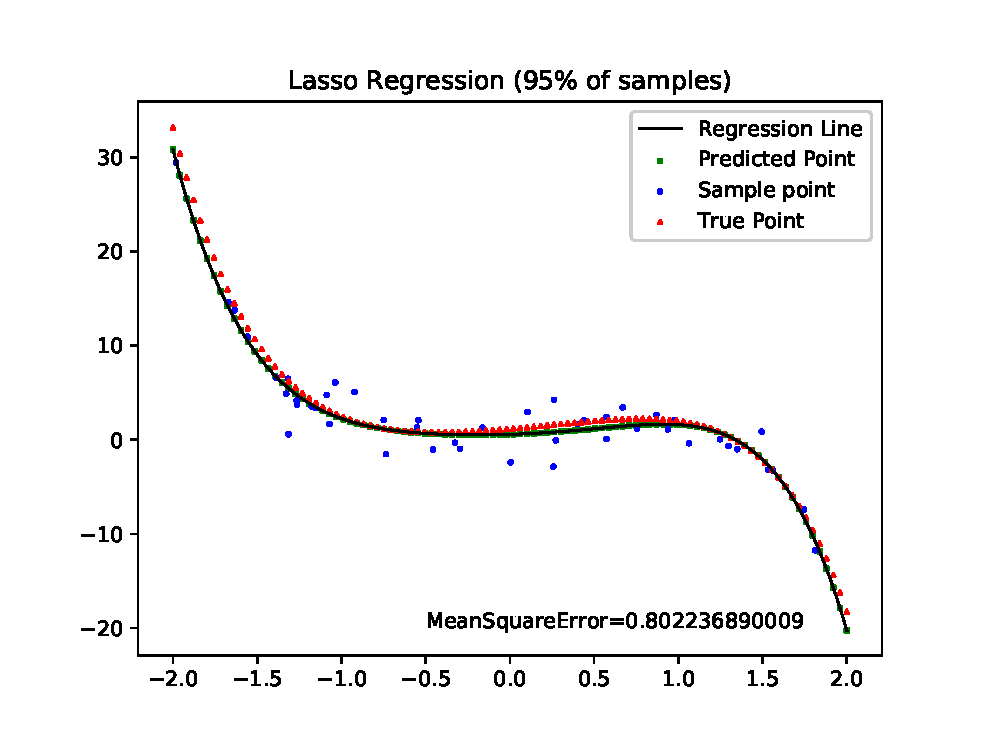
\includegraphics[width=.9\linewidth]{LassoRegression_outliers95.eps}
  	\caption{95\%}
\end{subfigure}
	\caption{Lasso Regression}
\end{figure}

\begin{figure}[H]
\centering
\begin{subfigure}{.18\textwidth}
  	\centering
  	\includegraphics[width=.9\linewidth]{LeastSquareRegression_outliers15.eps}
  	\caption{15\%}
\end{subfigure}%
\begin{subfigure}{.18\textwidth}
  	\centering
  	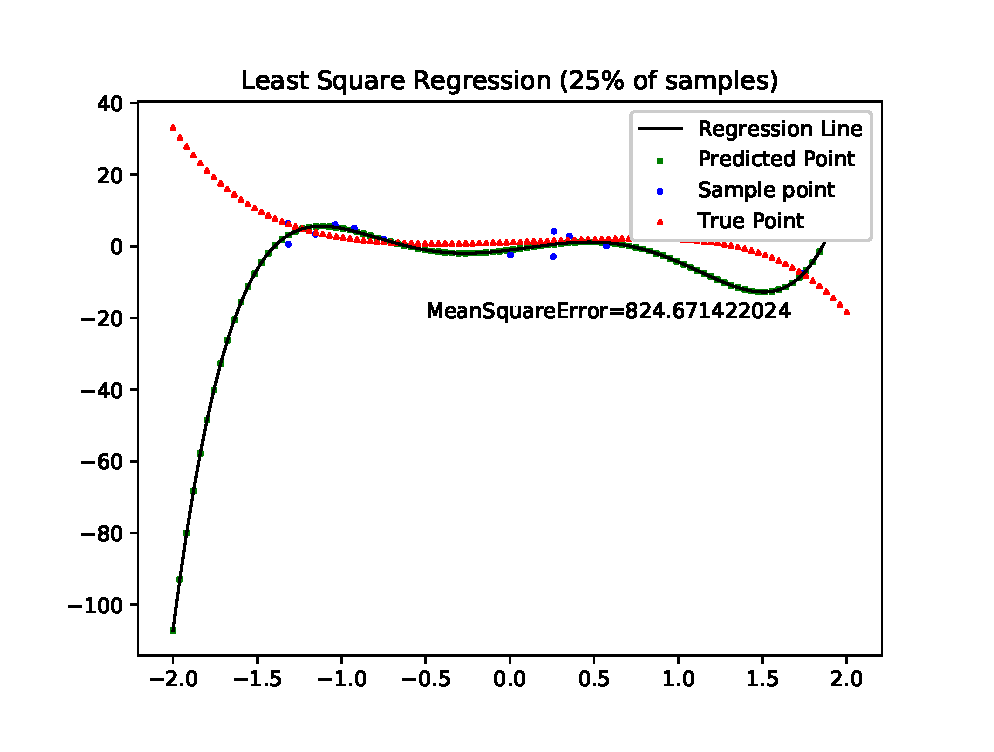
\includegraphics[width=.9\linewidth]{LeastSquareRegression_outliers25.eps}
  	\caption{25\%}
\end{subfigure}%
\begin{subfigure}{.18\textwidth}
  	\centering
  	\includegraphics[width=.9\linewidth]{LeastSquareRegression_outliers35.eps}
  	\caption{35\%}
\end{subfigure}%
\begin{subfigure}{.18\textwidth}
  	\centering
  	\includegraphics[width=.9\linewidth]{LeastSquareRegression_outliers45.eps}
  	\caption{45\%}
\end{subfigure}
\begin{subfigure}{.18\textwidth}
  	\centering
  	\includegraphics[width=.9\linewidth]{LeastSquareRegression_outliers55.eps}
  	\caption{55\%}
\end{subfigure}%
\begin{subfigure}{.18\textwidth}
  	\centering
  	\includegraphics[width=.9\linewidth]{LeastSquareRegression_outliers65.eps}
  	\caption{65\%}
\end{subfigure}%
\begin{subfigure}{.18\textwidth}
  	\centering
  	\includegraphics[width=.9\linewidth]{LeastSquareRegression_outliers75.eps}
  	\caption{75\%}
\end{subfigure}%
\begin{subfigure}{.18\textwidth}
  	\centering
  	\includegraphics[width=.9\linewidth]{LeastSquareRegression_outliers85.eps}
  	\caption{85\%}
\end{subfigure}%
\begin{subfigure}{.18\textwidth}
  	\centering
  	\includegraphics[width=.9\linewidth]{LeastSquareRegression_outliers95.eps}
  	\caption{95\%}
\end{subfigure}
	\caption{Least Square Regression}
\end{figure}


\begin{figure}[H]
\centering
\begin{subfigure}{.18\textwidth}
  	\centering
  	\includegraphics[width=.9\linewidth]{RegularizedLSRegression_outliers15.eps}
  	\caption{15\%}
\end{subfigure}%
\begin{subfigure}{.18\textwidth}
  	\centering
  	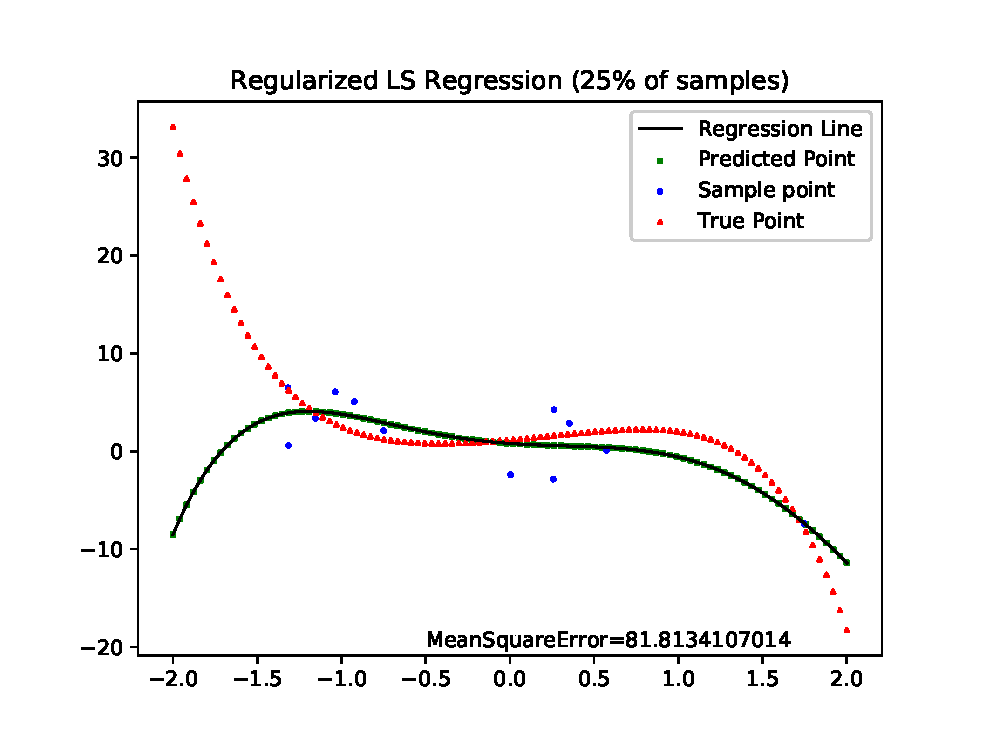
\includegraphics[width=.9\linewidth]{RegularizedLSRegression_outliers25.eps}
  	\caption{25\%}
\end{subfigure}%
\begin{subfigure}{.18\textwidth}
  	\centering
  	\includegraphics[width=.9\linewidth]{RegularizedLSRegression_outliers35.eps}
  	\caption{35\%}
\end{subfigure}%
\begin{subfigure}{.18\textwidth}
  	\centering
  	\includegraphics[width=.9\linewidth]{RegularizedLSRegression_outliers45.eps}
  	\caption{45\%}
\end{subfigure}
\begin{subfigure}{.18\textwidth}
  	\centering
  	\includegraphics[width=.9\linewidth]{RegularizedLSRegression_outliers55.eps}
  	\caption{55\%}
\end{subfigure}%
\begin{subfigure}{.18\textwidth}
  	\centering
  	\includegraphics[width=.9\linewidth]{RegularizedLSRegression_outliers65.eps}
  	\caption{65\%}
\end{subfigure}%
\begin{subfigure}{.18\textwidth}
  	\centering
  	\includegraphics[width=.9\linewidth]{RegularizedLSRegression_outliers75.eps}
  	\caption{75\%}
\end{subfigure}%
\begin{subfigure}{.18\textwidth}
  	\centering
  	\includegraphics[width=.9\linewidth]{RegularizedLSRegression_outliers85.eps}
  	\caption{85\%}
\end{subfigure}%
\begin{subfigure}{.18\textwidth}
  	\centering
  	\includegraphics[width=.9\linewidth]{RegularizedLSRegression_outliers95.eps}
  	\caption{95\%}
\end{subfigure}
	\caption{Regularized LS Regression}
\end{figure}



\begin{figure}[H]
\centering
\begin{subfigure}{.18\textwidth}
  	\centering
  	\includegraphics[width=.9\linewidth]{RobustRegression_outliers15.eps}
  	\caption{15\%}
\end{subfigure}%
\begin{subfigure}{.18\textwidth}
  	\centering
  	\includegraphics[width=.9\linewidth]{RobustRegression_outliers25.eps}
  	\caption{25\%}
\end{subfigure}%
\begin{subfigure}{.18\textwidth}
  	\centering
  	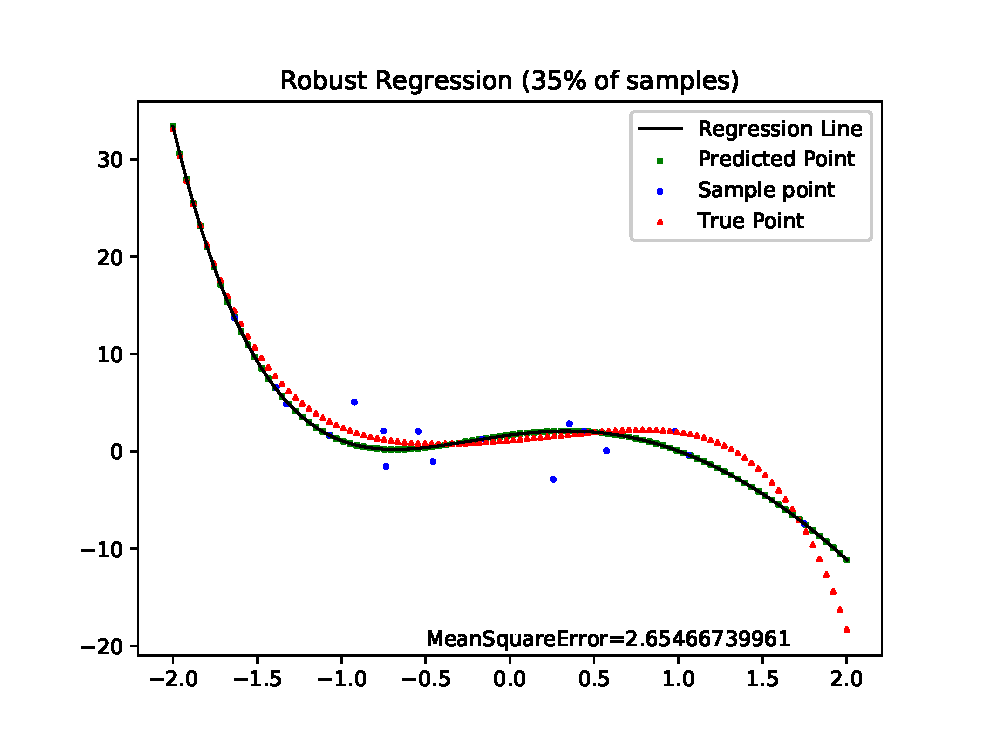
\includegraphics[width=.9\linewidth]{RobustRegression_outliers35.eps}
  	\caption{35\%}
\end{subfigure}%
\begin{subfigure}{.18\textwidth}
  	\centering
  	\includegraphics[width=.9\linewidth]{RobustRegression_outliers45.eps}
  	\caption{45\%}
\end{subfigure}
\begin{subfigure}{.18\textwidth}
  	\centering
  	\includegraphics[width=.9\linewidth]{RobustRegression_outliers55.eps}
  	\caption{55\%}
\end{subfigure}%
\begin{subfigure}{.18\textwidth}
  	\centering
  	\includegraphics[width=.9\linewidth]{RobustRegression_outliers65.eps}
  	\caption{65\%}
\end{subfigure}%
\begin{subfigure}{.18\textwidth}
  	\centering
  	\includegraphics[width=.9\linewidth]{RobustRegression_outliers75.eps}
  	\caption{75\%}
\end{subfigure}%
\begin{subfigure}{.18\textwidth}
  	\centering
  	\includegraphics[width=.9\linewidth]{RobustRegression_outliers85.eps}
  	\caption{85\%}
\end{subfigure}%
\begin{subfigure}{.18\textwidth}
  	\centering
  	\includegraphics[width=.9\linewidth]{RobustRegression_outliers95.eps}
  	\caption{95\%}
\end{subfigure}
	\caption{Robust Regression}
\end{figure}



Figure \ref{fig:ts} on the above shows the average error in 2000 times versus training size; as we can see from the figure, Least-squares Regression and Robust Regression more robust with less data (only around 20\% of the sample) while the other tend to overfit badly when the size of sample is less 50\%.
 \begin{figure}[H]
\centering
\begin{subfigure}{.3\textwidth}
  	\centering
  	\includegraphics[width=.9\linewidth]{BayessianRegressionsubseterror.eps}
  	\caption{Bayesian Regression}
\end{subfigure}%
\begin{subfigure}{.3\textwidth}
  	\centering
  	\includegraphics[width=.9\linewidth]{LassoRegressionsubseterror.eps}
  	\caption{Lasso Regression}
\end{subfigure}
\begin{subfigure}{.3\textwidth}
  	\centering
  	\includegraphics[width=.9\linewidth]{RegularizedLSRegressionsubseterror.eps}
  	\caption{Regularized LS Regression}
\end{subfigure}%
\begin{subfigure}{.3\textwidth}
  	\centering
  	\includegraphics[width=.9\linewidth]{LeastSquaresRegressionsubseterror.eps}
  	\caption{Least Square Regression}
\end{subfigure}%
\begin{subfigure}{.3\textwidth}
  	\centering
  	\includegraphics[width=.9\linewidth]{RobustRegressionsubseterror.eps}
  	\caption{Robust Regression}
\end{subfigure}

	\caption{Mean-squared Error versus Training Size}
	\label{fig:ts}
\end{figure}

\subsection{Regression and Prediction on Samples with Outliers}
In this experiment, I added a random integer (can be negative or positive) with range from 20 to 30 to 15\% of training samples. Figure \ref{fig:out} shows that Robust Regression are robust to the presence of outliers because whose MSE value is merely 1 while the MSEs of the other 4 algorithms reach more than 10. Among 5 algorithm, Least Square Regression whose MSE are the largest are most sensitive to the outliers.


\begin{table}[htp]
\caption{Mean Square Error on Sample with Outliers}
\begin{center}
\begin{tabular}{|c|c|}
\hline
		Algorithm  &  MSE \\
\hline	
		Least Square    &  13.7723 \\
		Regularized LS &  10.0730 \\
		Lasso		&  13.7718 \\
		\textbf{Robust}	&  1.01940 \\
		Bayesian 		&  10.1678 \\
\hline
\end{tabular}
\end{center}
\label{default}
\end{table}%


\begin{figure}[H]
\centering
\begin{subfigure}{.3\textwidth}
  	\centering
  	\includegraphics[width=.9\linewidth]{RobustRegression_outliers.eps}
  	\caption{Robust Regression}
\end{subfigure}%
\begin{subfigure}{.3\textwidth}
  	\centering
  	\includegraphics[width=.9\linewidth]{BayesianRegression_outliers.eps}
  	\caption{Bayesian Regression}
\end{subfigure}
\begin{subfigure}{.3\textwidth}
  	\centering
  	\includegraphics[width=.9\linewidth]{LassoRegression_outliers.eps}
  	\caption{Lasso Regression}
\end{subfigure}%
\begin{subfigure}{.3\textwidth}
  	\centering
  	\includegraphics[width=.9\linewidth]{RegularizedLSRegression_outliers.eps}
  	\caption{Regularized LS Regression}
\end{subfigure}%
\begin{subfigure}{.3\textwidth}
  	\centering
  	\includegraphics[width=.9\linewidth]{LeastSquareRegression_outliers.eps}
  	\caption{Least Square Regression}
\end{subfigure}

	\caption{Regression and Prediction on Sample with Outliers}
	\label{fig:out}
\end{figure}

\subsection{Higher-order Polynomial Estimation}

In this section, I used the sample data (sampx, sampy) to estimate the parameters of a 10th order polynomial function for each regression method. 
\begin{table}[H]
\caption{Mean Square Error on 10th order}
\begin{center}
\begin{tabular}{|c|c|}
\hline
		Algorithm  &  MSE \\
\hline	
		Least Square    &  13.7723 \\
		Regularized LS &  10.0730 \\
		Lasso		&  13.7718 \\
		\textbf{Robust}	&  1.01940 \\
		Bayesian 		&  10.1678 \\
\hline
\end{tabular}
\end{center}
\label{d}
\end{table}%
The Table \ref{d} shows that Robust Regression has the least mean-squared error, however in the figure \label{fig:10order} it seems that RR is well-fitting than the other models. The reason why RR has the best MSE is that the other 4 models overfitted the tail of samples (polyx $> 1.5$ ) badly which cause the average bad performance on the whole sample. Also figure \label{fig:10order} shows the prediction of Bayesian Regression is the most overfitting with the highest mean-squared error that results from the worst overfitting on the tail of the sample.


\begin{figure}[H]
\centering

\begin{subfigure}{.3\textwidth}
  	\centering
  	\includegraphics[width=.9\linewidth]{BayessianRegression_10thorder.eps}
  	\caption{Bayesian Regression}
\end{subfigure}%
\begin{subfigure}{.3\textwidth}
  	\centering
  	\includegraphics[width=.9\linewidth]{LassoRegression_10thorder.eps}
  	\caption{Lasso Regression}
\end{subfigure}
\begin{subfigure}{.3\textwidth}
  	\centering
  	\includegraphics[width=.9\linewidth]{RegularizedLSRegression_10thorder.eps}
  	\caption{Regularized LS Regression}
\end{subfigure}%
\begin{subfigure}{.3\textwidth}
  	\centering
  	\includegraphics[width=.9\linewidth]{RobustRegression_10thorder.eps}
  	\caption{Robust Regression}
\end{subfigure}%
\begin{subfigure}{.3\textwidth}
  	\centering
  	\includegraphics[width=.9\linewidth]{LeastSquareRegression_10thorder.eps}
  	\caption{Least Square Regression}
\end{subfigure}

	\caption{Regression and Prediction on Sample with Outliers}
	\label{fig:10order}
\end{figure}


\subsection{Conclusion}
After the above experiments, I found that among 5 algorithm Robust Regression had the worst performance in the texting though, it achieved the best performance in the experiments with less training data or adding outliers, which means that Robust Regression is indeed more "Robust" than other method and has less chance to be overfitting. On the other hand, I found that the performance of Lasso and Least-squares Regression are easy to be disturbed by outliers and less training data, which means they have the high risk to be overfitting in bad training dataset.



\section{A real world regression problem - counting people}
\subsection{Number of People Prediction on Original Feature}


In this section, I use the feature directly (set $\phi(x) = x$). Table \ref{cp1} and Figure \ref{fig:cp1p} show that Regularized LS Regression works the best with the lowest mean-absolute error (MAE=1.2794) and mean-squared error (MSE=2.6503).


\begin{table}[H]
\caption{Error on People Counting Prediction using Original Features}
\begin{center}
\begin{tabular}{|c|c|c|}
\hline
		Algorithm  &  MSE  &  MAE\\
\hline	
		Least Square    &  3.1028  	& 1.3584\\
		\textbf{Regularized LS} &  2.6503 		&1.2794\\
		Lasso		&  3.1027 		&1.3584\\
		Robust	&  3.1189 		&1.3645\\
		Bayesian 		&  2.6552		&1.2801\\
\hline
\end{tabular}
\end{center}
\label{cp1}
\end{table}%


\begin{figure}[H]
\centering

\begin{subfigure}{.3\textwidth}
  	\centering
  	\includegraphics[width=.9\linewidth]{bayessian_cp_1phi.eps}
  	\caption{Bayesian Regression}
\end{subfigure}%
\begin{subfigure}{.3\textwidth}
  	\centering
  	\includegraphics[width=.9\linewidth]{lasso_cp_1phi.eps}
  	\caption{Lasso Regression}
\end{subfigure}
\begin{subfigure}{.3\textwidth}
  	\centering
  	\includegraphics[width=.9\linewidth]{rls_cp_1phi.eps}
  	\caption{Regularized LS Regression}
\end{subfigure}%
\begin{subfigure}{.3\textwidth}
  	\centering
  	\includegraphics[width=.9\linewidth]{rr_cp_1phi.eps}
  	\caption{Robust Regression}
\end{subfigure}%
\begin{subfigure}{.3\textwidth}
  	\centering
  	\includegraphics[width=.9\linewidth]{ls_cp_1phi.eps}
  	\caption{Least Square Regression}
\end{subfigure}

	\caption{People Counting Prediction on Original Features}
	\label{fig:cp1p}
\end{figure}


\subsection{Number of People Prediction on Transformed Feature}
\subsubsection{2nd Order Polynomial Transformed Feature}
Here I created a simple 2nd order polynomial as $\phi(x) = [x_1,\dots, x_9, x_1^2, \dots ,x_9^2]$. Table \ref{cp2} and Figure \ref{fig:cp2p} show that all 5 regression model achieved better performance with the 2nd order polynomial transformed feature and  Regularized LS Regression still works the best.


\begin{table}[H]
\caption{Error on People Counting Prediction using 2nd Order Polynomial Features}
\begin{center}
\begin{tabular}{|c|c|c|}
\hline
		Algorithm  &  MSE  &  MAE\\
\hline	
		Least Square    &  2.9235  	& 1.3267\\
		\textbf{Regularized LS} &  2.4277 		&1.2088\\
		Lasso		&  2.9235 		&1.3267\\
		Robust	&  2.8981 		&1.3079\\
		Bayesian 		&  2.4293		&1.2094\\
\hline
\end{tabular}
\end{center}
\label{cp2}
\end{table}%

\begin{figure}[H]
\centering
\begin{subfigure}{.3\textwidth}
  	\centering
  	\includegraphics[width=.9\linewidth]{bayessian_cp_2phi.eps}
  	\caption{Bayesian Regression}
\end{subfigure}%
\begin{subfigure}{.3\textwidth}
  	\centering
  	\includegraphics[width=.9\linewidth]{lasso_cp_2phi.eps}
  	\caption{Lasso Regression}
\end{subfigure}
\begin{subfigure}{.3\textwidth}
  	\centering
  	\includegraphics[width=.9\linewidth]{rls_cp_2phi.eps}
  	\caption{Regularized LS Regression}
\end{subfigure}%
\begin{subfigure}{.3\textwidth}
  	\centering
  	\includegraphics[width=.9\linewidth]{rr_cp_2phi.eps}
  	\caption{Robust Regression}
\end{subfigure}%
\begin{subfigure}{.3\textwidth}
  	\centering
  	\includegraphics[width=.9\linewidth]{ls_cp_2phi.eps}
  	\caption{Least Square Regression}
\end{subfigure}

	\caption{People Counting Prediction on 2nd Order Polynomial Features}
	\label{fig:cp2p}
\end{figure}

\subsubsection{2nd \& 3rd Order Polynomial Transformed Feature}
Here I created a combination with 2nd order polynomial and  3rd order polynomial as $\phi(x) = [x_1,\dots, x_9, x_1^2, \dots ,x_9^2,  x_1^3, \dots ,x_9^3]$. Table \ref{cp2} for people counting prediction. Figure \ref{fig:cp2p} show that only Bayesian Regression achieved obviously better performance. As a result, Bayesian Regression merely works best among 5 methods.
\begin{table}[H]
\caption{Error on People Counting Prediction using 2nd Order Polynomial Features}
\begin{center}
\begin{tabular}{|c|c|c|}
\hline
		Algorithm  &  MSE  &  MAE\\
\hline	
		Least Square    &  2.9282 	& 1.3191\\
		Regularized LS &  2.4640 		&1.2369\\
		Lasso		&  2.9235 		&1.3267\\
		Robust	&  3.1116 		&1.3517\\
		\textbf{Bayesian} 		&  2.4619		&1.2359\\
\hline
\end{tabular}
\end{center}
\label{cp2}
\end{table}%
\begin{figure}[H]
\centering
\begin{subfigure}{.3\textwidth}
  	\centering
  	\includegraphics[width=.9\linewidth]{bayessian_cp_3phi.eps}
  	\caption{Bayesian Regression}
\end{subfigure}%
\begin{subfigure}{.3\textwidth}
  	\centering
  	\includegraphics[width=.9\linewidth]{lasso_cp_3phi.eps}
  	\caption{Lasso Regression}
\end{subfigure}
\begin{subfigure}{.3\textwidth}
  	\centering
  	\includegraphics[width=.9\linewidth]{rls_cp_3phi.eps}
  	\caption{Regularized LS Regression}
\end{subfigure}%
\begin{subfigure}{.3\textwidth}
  	\centering
  	\includegraphics[width=.9\linewidth]{rr_cp_3phi.eps}
  	\caption{Robust Regression}
\end{subfigure}%
\begin{subfigure}{.3\textwidth}
  	\centering
  	\includegraphics[width=.9\linewidth]{ls_cp_3phi.eps}
  	\caption{Least Square Regression}
\end{subfigure}

	\caption{People Counting Prediction on 2nd \& 3rd Order Polynomial Features}
	\label{fig:cp2p}
\end{figure}

\subsection{Conclusion}
Regularized LS Regression achieved the best performance on people counting prediction. With 2nd Order and 2nd Order\& 3rd Order Polynomial feature transformation, all 5 regression methods achieved better performance than using original feature. Under 3rd Order Polynomial feature transformation, Bayesian Regression had highest effect enhancement.


\end{document}  